% Template for Cogsci submission with R Markdown

% Stuff changed from original Markdown PLOS Template
\documentclass[10pt, letterpaper]{article}

\usepackage{cogsci}
\usepackage{pslatex}
\usepackage{float}
\usepackage{caption}

% amsmath package, useful for mathematical formulas
\usepackage{amsmath}

% amssymb package, useful for mathematical symbols
\usepackage{amssymb}

% hyperref package, useful for hyperlinks
\usepackage{hyperref}

% graphicx package, useful for including eps and pdf graphics
% include graphics with the command \includegraphics
\usepackage{graphicx}

% Sweave(-like)
\usepackage{fancyvrb}
\DefineVerbatimEnvironment{Sinput}{Verbatim}{fontshape=sl}
\DefineVerbatimEnvironment{Soutput}{Verbatim}{}
\DefineVerbatimEnvironment{Scode}{Verbatim}{fontshape=sl}
\newenvironment{Schunk}{}{}
\DefineVerbatimEnvironment{Code}{Verbatim}{}
\DefineVerbatimEnvironment{CodeInput}{Verbatim}{fontshape=sl}
\DefineVerbatimEnvironment{CodeOutput}{Verbatim}{}
\newenvironment{CodeChunk}{}{}

% cite package, to clean up citations in the main text. Do not remove.
\usepackage{apacite}

% KM added 1/4/18 to allow control of blind submission
\cogscifinalcopy

\usepackage{color}

% Use doublespacing - comment out for single spacing
%\usepackage{setspace}
%\doublespacing


% % Text layout
% \topmargin 0.0cm
% \oddsidemargin 0.5cm
% \evensidemargin 0.5cm
% \textwidth 16cm
% \textheight 21cm

\title{Predicting Early Language Development with Linguistic Alignment}


\author{{\large \bf Joseph Denby} \\ Department of Psychology \\ University of Chicago \\ \texttt{jgdenby@uchicago.edu} \And {\large \bf Daniel Yurovsky} \\ Department of Psychology\\ University of Chicago \\\texttt{yurovsky@uchicago.edu}}

\begin{document}

\maketitle

\begin{abstract}
Children are capable of quickly gaining enormous linguistic knowledge
during early development, in part due to low-level features of their
parents' speech. Some posit that parents contribute to their child's
language development by calibrating their language according to their
child's developmental abilities and needs. Here, we investigate this
hypothesis by conducting a statistical analysis of this `linguistic
alignment' in a large-scale corpus of parent-child conversations
recorded over a period of 5 years. Our results corroborate previous
findings, showing strong parental alignment that slowly decreases as
children mature; in addition, we demonstrate the impact of alignment on
development by linking its effects with development outcome measures.

\textbf{Keywords:}
Language acquisition; computational modeling; cognitive development
\end{abstract}

\hypertarget{introduction}{%
\section{Introduction}\label{introduction}}

Children make vast linguistic strides within their first few years of
life, rapidly growing their vocabulary (Mayor \& Plunkett, 2010) and
acquiring an understanding of compositional structure (Lieven, Salomo,
\& Tomasello, 2009).To explore this feat, many have probed the role of
statistical learning in features of language development, such as
detecting words (Saffran, Aslin, \& Newport, 1996), grammar (Gomez \&
Gerken, 1999), and semantics (Naigles, 1990; Smith \& Yu, 2008; Yuan \&
Fisher, 2009).

As a supplement to this line of inquiry, others have put forward the
linguistic tuning hypothesis, arguing that parents bolster their child's
early language learning by calibrating the complexity of their speech to
the particular abilities and needs of their children (Montag \&
MacDonald, 2015; Snow, 1972; Thiessen, Hill, \& Saffran, 2005). The idea
is intuitive, but it is unclear at what level tuning occurs (Hayes \&
Ahrens, 1988; Sokolov, 1993; Spivey \& Dale, 2006) and how overt it is
(Brown \& Hanlon, 1970; Chouinard \& Clark, 2003; Hirsh-Pasek, Treiman,
\& Schneiderman, 1984).

A parallel yet complementary vein of language development research
investigates the presence of low-level cues in parental speech and their
influence on child language learning. From this research, we know that
child-directed speech contains features that facilitate language
learning, and that more exposure tends to result in better outcomes
(Cameron-Faulkner, Lieven, \& Tomasello, 2003; Weisleder \& Fernald,
2013). Related, caregivers from families of high socioeconomic status
(SES) tend to converse more with their children than their lower SES
counterparts, and these increases are associated with improved
development outcomes such as vocabulary size and school performance
(Walker, Greenwood, Hart, \& Carta, 1994; Walker et al., 1994).
Moreover, differences in SES-based language development are largely
explained by low-level features of parental child-directed speech such
as lexical diversity and sentence complexity (Hoff, 2003; Rowe, 2008).
So, given that granular aspects of parent speech can have substantial
effects on a child's language development, it may be that linguistic
tuning occurs at this level in subtle ways, particularly when it comes
to non-content words (i.e., words that are not central to the topic of
discussion.)

This idea of assessing the direct impact of a parent's usage of
non-content word on language development relates to linguistic
alignment, a phenomenon whereby conversational partners tend to align
aspects of their communicative style and content according to various
external influences e.g., (Pennebaker, Booth, Boyd, \& Francis, 2015).
Yurovsky, Doyle, \& Frank (2016) investigates linguistic alignment in
CHILDES (MacWhinney, 2000), a natural language corpus of conversation
between parents and children to assess whether tuning occurs at the
level of syntactic categories. They find that syntactic alignment does
occur between both parents and children; moreover, parents align less
over time, suggesting that the relationship their speech shares with
their child's changes as a function of development. These results
present a powerful proof of concept that syntactic alignment exists
between parents and children and changes over time, but it remains
unclear whether alignment bears any sort of concrete, impactful
relationship to language development.

Here, we extend the Yurovsky, Doyle, \& Frank (2016) model by applying
it to the Language Development Project (LDP) (Goldin-Meadow et al.,
2014), a corpus of ecological conversations between parents and their
children over time, collected from a socioeconomically diverse sample of
parent-child dyads. Moreover, we use alignment estimates alongside
demographic information to predict language outcome measures,
strengthening the linguistic tuning hypothesis by concretely showing how
parents' sensitivity to their child's linguistic needs and abilities
impacts their development.

\hypertarget{model}{%
\section{Model}\label{model}}

The linguistic tuning hypothesis predicts that parents will calibrate
their language in part by assessing their child's needs and abilities.
So, we predict that parents will exhibit high alignment to their young
children, but will reduce their alignment as their children mature. To
test this prediction, we employ an extended version of the Hierarchical
Alignment Model (HAM) implemented in Yurovsky et al. (2016) which both
estimates the impact of a speaker's use of syntactic categories on their
conversational partner's usage and uses these alignment estimates to
predict language outcome scores.

At base, the model predicts, for each utterance, whether the speaker
will produce a word from a given syntactic category. This prediction is
generated by two factors: the speaker's baseline propensity towards
using that category and the speaker's tendency to align, producing words
from a category just used by their partner. In the model, the primary
computation mimics a standard logistic regression - the production of a
syntactic category within an utterance is treated as a binary outcome
variable impacted by a linear combination of predictor variables (here,
baseline usage and alignment.) The model's hierarchical structure then
allows the estimates of baseline usage and alignment effects to be
pooled across individual speakers and syntactic categories in a way that
ensures statistical robustness.

The model used here then incorporates these alignment and baseline usage
estimates as predictors in a linear regression model of PPVT (Dunn \&
Dunn, 1997). At this stage, PPVT is estimated as a linear combination of
predictors reflecting alignment and baseline usage estimate for both
parents and children alongside other predictors representing demographic
variables (e.g., child's gender, mother's education) and the child's
age.

\begin{table}[H]
\centering
\begin{tabular}{rll}
  \hline
 & category & examples \\ 
  \hline
1 & article & a, alot \\ 
  2 & certain & altogether, must \\ 
  3 & conj & but, or \\ 
  4 & discrep & wanted, hoped \\ 
  5 & excl & whether, not \\ 
  6 & i & i'm, i \\ 
  7 & incl & both, around \\ 
  8 & ipron & thatd, whats \\ 
  9 & negate & needn't, oughtn't \\ 
  10 & preps & at, to \\ 
  11 & quant & series, every \\ 
  12 & tentat & anyhow, most \\ 
  13 & we & we'd, lets \\ 
  14 & you & youd, y'all \\ 
   \hline
\end{tabular}
\caption{LIWC Categories with example words.} 
\end{table}

\hypertarget{model-details}{%
\subsection{Model Details}\label{model-details}}

The structure of the model used here greatly resembles that used in
Yurovsky et al. (2016), in that it operates over utterances represented
as binary vectors, with indices indicating the presence or absence of
each of the 14 LIWC categories. The probability of producing each
category in each utterance is predicted from two parameters: the
speaker's baseline usage of that syntactic category (\(\eta^{base}\)),
and the change in that speaker's baseline as a function of interacting
with the listener (\(\eta^{align}\)). So, for a given syntactic category
\(c\), for replies to utterances that don't contain \(c\), the
production parameter for that category is computed by applying the
inverse logit function to the appropriate baseline log odds: \[
P(Production_c) = logit^{-1}(\eta^{base}_c)
\] Alternatively, replies to utterances that \emph{do} contain \(c\),
the parameter computation takes into account the sum of the baseline and
alignment log odds: \[
P(Production_c) = logit^{-1}(\eta^{base}_c+\eta^{align}_c)
\]

To accommodate the variance in production across the LIWC categories,
each baseline usage parameter was drawn from an uninformative prior
(\(\eta^{base} \sim Uniform(-5,5)\)); alignment parameters were
regularized towards 0 by way of implementing a conservative prior
(\(\eta^{align} \sim Normal(0,1)\)).

All parameters were estimated hierarchically, which allows intelligent
pooling of data across participants in the dataset. Each subpopulation
(i.e., all parents and all children) obtained an alignment estimate,
each of which produced speaker-level alignment estimates, which produced
category-level alignment estimates. The order was flipped for baseline
parameters in order to better reflect empirical baseline usages across
syntactic categories; subpopulation estimates produced category-level
estimates, which then produced speaker-level estimates. As in Yurovsky
et al. (2016), we also include parameters that allow baseline
(\(\beta\)) and alignment probabilities (\(\alpha\)) to change linearly
over time.

Next, we extend the model used in Yurovsky et al. (2016) by using
estimated alignment (i.e., \(\eta\) parameters) to predict PPVT scores,
a widely used inventory for tracking language development (Dunn \& Dunn,
1997). To do so, we implement a regression model where PPVT scores are
modeled as linear combinations of various predictor variables. These
predictor variables included the child's age, alignment parameter
estimates for the child and their parent, the mother's education, the
child's gender, as well as interaction effects for all variables with
age. The error variance for this model was estimated using parameter
\(\sigma\).

The model implemented here then serves two purposes: (1) It extends the
analysis of Yurovsky et al. (2016) to a new dataset, aiming to replicate
previous findings in a more diverse and representative sample, and (2)
It incorporates alignment estimates in a predictive model of early
language outcomes, serving to test the hypothesis that alignment has
significant effects on language development over and above demographic
features. To be specific, we hope to replicate non-zero estimates for
\(\eta\) parameters (demonstrating that alignment between parents and
children exists across datasets), positive \(\beta\) for children
(showing that children increase their baseline usage of categories over
time), and negative \(\alpha\) for parents (showing that parents
decrease their alignment as their children age.) If the PPVT model
estimates for parameters corresponding to the main or interaction
effects of alignment are non-zero in the presence of demographic
variables, we can infer that alignment has a significant effect on early
language development.

\begin{CodeChunk}
\begin{figure}[H]
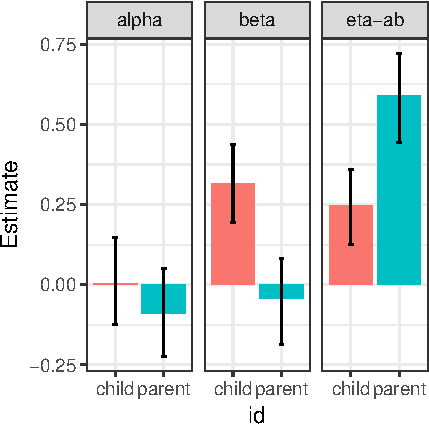
\includegraphics{figs/plot-1} \caption[This plot is not beautiful yet]{This plot is not beautiful yet.}\label{fig:plot}
\end{figure}
\end{CodeChunk}

\hypertarget{analysis}{%
\section{Analysis}\label{analysis}}

\hypertarget{data-and-methodology}{%
\subsection{Data and Methodology}\label{data-and-methodology}}

Transcripts were sourced from the Language Development Project corpus
(Goldin-Meadow et al., 2014), consisting of conversations between 62
child-parent pairs spanning 12 to 60 months of age. This corpus amounts
to 712 total transcripts with a median representation of \(12\) sessions
per subject pair. The sample includes 30 female children and large
representation of socioeconomic status based on the mother's level of
education: 22 with an advanced degree, 20 with a bachelor's degree, 10
with some college or trade school, 8 with a high school degree or GED,
and 2 with some high school.

Following Yurovsky et al. (2016), successive utterances from a speaker
within a transcript were concatenated into a single utterance.
Individual utterances were then transformed into a binary vector with
indices indicating the presence or absence of each of the 14 LIWC
categories. This pre-processing turned every transcript into a
speaker-reply format: each utterance within a transcript was both a
reply to the preceding utterance and a message to the next one.

Each transcript was then compressed, yielding 4 numbers for each LIWC
category. For a pair of speakers \emph{A} and \emph{B} in a transcript,
for each LIWC category, we computed the number of utterances from
\emph{A} to \emph{B} containing the category (\(N^{align}\)), the number
of utterances from \emph{A} to \emph{B} not containing the category
(\(N^{base}\)), the number of utterances containing the category
responding to an utterance containing the category (\(C^{align}\)), and
the number of utterances containing the category responding to an
utterance not containing the category (\(C^{base}\)). Aggregating in
this way provided the platform for the model's sampling - for each
transcript, \(C^{base}\) and \(C^{align}\) were drawn from Binomial
distributions parameterized by \(N^{base}\) and \(N^{align}\) chances
respectively, with probabilities computed via the logistic regression
models outlined above.\\
Sampling was performed using Stan, a probabilistic programming language
that implements Hamiltonian Monte Carlo sampling methods (Carpenter et
al., 2017). Posterior distributions for each parameter in the model were
estimated using 350 iterations (THIS WILL LIKELY CHANGE).
\footnote{Code available at \texttt{https://github.com/callab/ldp-alignment}}

\begin{CodeChunk}
\begin{figure*}[h]

{\centering 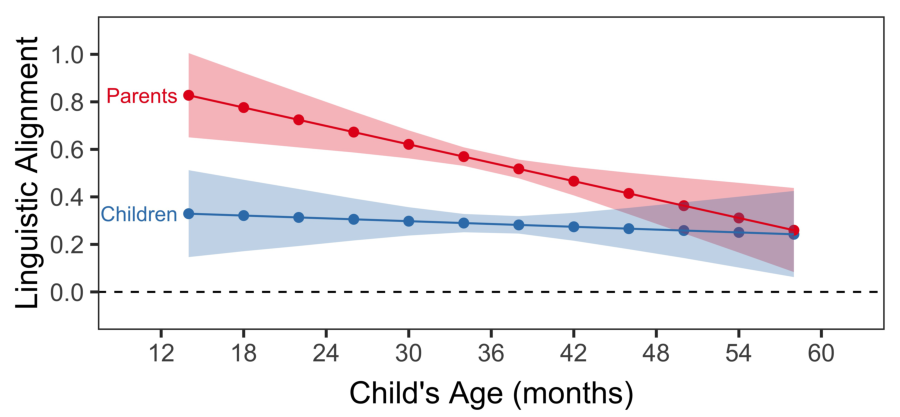
\includegraphics{figs/2-col-image-1} 

}

\caption[This is not the right plot but it is close]{This is not the right plot but it is close.}\label{fig:2-col-image}
\end{figure*}
\end{CodeChunk}

\hypertarget{results}{%
\subsection{Results}\label{results}}

Alignment estimates (\(\eta^{align}\)) for parents and children were
both significantly above zero, corroborating the findings of Yurovsky et
al. (2016) in showing that both groups exhibit alignment (Figure 1). We
also replicate the finding that parents appear to align more to their
children than children align to their parents. The model estimates
developmental baseline changes (\(\beta\)) at approximately zero for
parents, but significantly above zero for children, replicating previous
findings. Alignment is estimated as having no significant age effect
(\(\alpha\)) in this dataset, failing to replicate the early finding
that parents tend to exhibit decreased alignment over their child's
development. However, the mean estimate is trending negatively,
suggesting this may be a function of the data's limited scope (Figure
2).

The estimates for PPVT predictors are listed alongside their standard
errors in Table 1. In our results, PPVT is positively associated with
the age of the child, the level of education of their mother, and their
being female. Moreover, female children tend to have a decreased age
effect on PPVT; this means that for female children, the expected
increase in PPVT over time is less stark (EXACT EFFECTS ARE DEPENDENT ON
FIT RESULTS). Alongside these demographic effects, we see some robust
alignment effects on PPVT: child alignment is associated with increased
PPVT, but a decreased age effect, while parental alignment is associated
with decreased PPVT and a decreased age effect.

\begin{table}[H]
\centering
\begin{tabular}{rlrr}
  \hline
 & measure & Estimate & StandardError \\ 
  \hline
1 & Age (years) & 23.62 & 3.09 \\ 
  2 & Child Alignment & 101.42 & 4.86 \\ 
  3 & Age x Child Alignment & -34.65 & 2.19 \\ 
  4 & Female & 0.76 & 3.85 \\ 
  5 & Age x Female & -1.02 & 1.62 \\ 
  6 & Intercept & -30.95 & 6.89 \\ 
  7 & Mother's Education & -0.84 & 1.10 \\ 
  8 & Age x Mother's Education & 3.61 & 0.36 \\ 
  9 & Parent Alignment & -20.86 & 6.96 \\ 
  10 & Age x Parent Alignment & -10.20 & 2.45 \\ 
  11 & $\sigma$ & 4.60 & 0.01 \\ 
   \hline
\end{tabular}
\caption{Parameter Estimates for PPVT predictors with standard errors.} 
\end{table}

\hypertarget{discussion}{%
\section{Discussion}\label{discussion}}

In an effort to understand and investigate how children rapidly acquire
language, some argue that the language parents produce to their children
is somehow calibrated to the child's particular needs and abilities
(Snow, 1972). While the idea is theoretically compelling, empirical work
has produced mixed results, with strong results in favor of (Chouinard
\& Clark, 2003; Hirsh-Pasek et al., 1984) and against (Brown \& Hanlon,
1970; Hayes \& Ahrens, 1988).

However, much of this prior work investigates tuning as an overt effort
on behalf of parents or tuning with respect to content words, with less
examining the potential role of low-level syntactic influence (Hoff,
2003). Yurovsky et al. (2016) presents just such an examination,
demonstrating using Bayesian hierarchical modeling that parents align to
their children according to their particular language usage at the level
of syntactic categories. This paper extends their model by applying it
to a new socioeconomically diverse sample of families (Goldin-Meadow et
al., 2014) and leveraging the model's alignment estimates to predict
language development outcomes.

The analysis presented here largely replicates the findings of Yurovsky
et al. (2016), showing strong alignment effects for both parents and
their children, a substantial age effect for baseline useage in
children, and a trending negative effect of age on alignment for
parents. Moreover, we demonstrate that these alignment estimates have
substantial power in predicting language development outcomes, even in
the presence of demographic features such as gender and socioeconomic
status. As such, these results serve to further the linguistic tuning
hypothesis, showing that alignment is a robust effect that appears to
have a relationship with language development independent of demographic
correlates.

\hypertarget{references}{%
\section{References}\label{references}}

\setlength{\parindent}{-0.1in} 
\setlength{\leftskip}{0.125in}

\noindent

\hypertarget{refs}{}
\leavevmode\hypertarget{ref-Brown:1970wd}{}%
Brown, R. W., \& Hanlon, C. (1970). Derivational Complexity and Order of
Acquisition in Child Speech. In J. Hayes (Ed.), \emph{Cognition and the
development of language} (pp. 11--53). New York.

\leavevmode\hypertarget{ref-CameronFaulkner:2003ge}{}%
Cameron-Faulkner, T., Lieven, E., \& Tomasello, M. (2003). A
construction based analysis of child directed speech. \emph{Cognitive
Science}, \emph{27}(6), 843--873.

\leavevmode\hypertarget{ref-Carpenter:2017ke}{}%
Carpenter, B., Gelman, A., Hoffman, M. D., Lee, D., Goodrich, B.,
Betancourt, M., \ldots{} Riddell, A. (2017). Stan : A Probabilistic
Programming Language. \emph{Journal of Statistical Software},
\emph{76}(1).

\leavevmode\hypertarget{ref-Chouinard:2003kq}{}%
Chouinard, M. M., \& Clark, E. V. (2003). Adult reformulations of child
errors as negative evidence. \emph{Journal of Child Language},
\emph{30}(3), 637--669.

\leavevmode\hypertarget{ref-PeabodyPictureVoca:im}{}%
Dunn, L. M., \& Dunn, L. M. (1997). Peabody Picture Vocabulary
Test--Third Edition. \emph{PsycTESTS Dataset}.

\leavevmode\hypertarget{ref-GoldinMeadow:2014hr}{}%
Goldin-Meadow, S., Levine, S. C., Hedges, L. V., Huttenlocher, J.,
Raudenbush, S. W., \& Small, S. L. (2014). New evidence about language
and cognitive development based on a longitudinal study: Hypotheses for
intervention. \emph{American Psychologist}, \emph{69}(6), 588--599.

\leavevmode\hypertarget{ref-Gomez:1999bx}{}%
Gomez, R. L., \& Gerken, L. (1999). Artificial grammar learning by
1-year-olds leads to specific and abstract knowledge. \emph{Cognition},
\emph{70}(2), 109--135.

\leavevmode\hypertarget{ref-Hayes:1988ue}{}%
Hayes, D. P., \& Ahrens, M. G. (1988). Vocabulary simplification for
children: a special case of 'motherese'? \emph{Journal of Child
Language}, \emph{15}(2), 395--410.

\leavevmode\hypertarget{ref-HirshPasek:1984bd}{}%
Hirsh-Pasek, K., Treiman, R., \& Schneiderman, M. (1984). Brown \&
Hanlon revisited: mothers' sensitivity to ungrammatical forms.
\emph{Journal of Child Language}, \emph{11}(01), 81--88.

\leavevmode\hypertarget{ref-Hoff:2003kx}{}%
Hoff, E. (2003). The specificity of environmental influence:
Socioeconomic status affects early vocabulary development via maternal
speech. \emph{Child Development}, \emph{74}(5), 1368--1378.

\leavevmode\hypertarget{ref-Lieven:2009ii}{}%
Lieven, E., Salomo, D., \& Tomasello, M. (2009). Two-year-old children's
production of multiword utterances: A usage-based analysis.
\emph{Cognitive Linguistics}, \emph{20}(3), 61--27.

\leavevmode\hypertarget{ref-MacWhinney:2000jx}{}%
MacWhinney, B. (2000). The CHILDES Project. \emph{Computational
Linguistics}, \emph{26}(4), 657--657.

\leavevmode\hypertarget{ref-Mayor:2010kp}{}%
Mayor, J., \& Plunkett, K. (2010). A statistical estimate of infant and
toddler vocabulary size from CDI analysis. \emph{Developmental Science},
\emph{14}(4), 769--785.

\leavevmode\hypertarget{ref-Montag:2015iy}{}%
Montag, J. L., \& MacDonald, M. C. (2015). Text exposure predicts spoken
production of complex sentences in 8- and 12-year-old children and
adults. \emph{Journal of Experimental Psychology: General},
\emph{144}(2), 447--468.

\leavevmode\hypertarget{ref-Naigles:1990cw}{}%
Naigles, L. (1990). Children use syntax to learn verb meanings.
\emph{Journal of Child Language}, \emph{17}(02), 357--374.

\leavevmode\hypertarget{ref-Pennebaker:kqtgxul0}{}%
Pennebaker, J. W., Booth, R. J., Boyd, R. L., \& Francis, M. E. (2015).
Linguistic inquiry and word count: LIWC2015. Austin, TX: Pennebaker
Conglomerates.

\leavevmode\hypertarget{ref-ROWE:2008go}{}%
Rowe, M. L. (2008). Child-directed speech: relation to socioeconomic
status, knowledge of child development and child vocabulary skill.
\emph{Journal of Child Language}, \emph{35}(01), 185--205.

\leavevmode\hypertarget{ref-Anonymous:6O2YEUCo}{}%
Saffran, J. R., Aslin, R. N., \& Newport, E. L. (1996). Statistical
Learning by 8-Month-Old Infants. \emph{Science}, \emph{274}(5294),
1926--1928.

\leavevmode\hypertarget{ref-Smith:2008gp}{}%
Smith, L., \& Yu, C. (2008). Infants rapidly learn word-referent
mappings via cross-situational statistics. \emph{Cognition},
\emph{106}(3), 1558--1568.

\leavevmode\hypertarget{ref-Snow:2018wf}{}%
Snow, C. E. (1972). Mothers' Speech to Children Learning Language.
\emph{Child Development}, \emph{43}(2), 549--565.

\leavevmode\hypertarget{ref-Sokolov:1993cr}{}%
Sokolov, J. L. (1993). A local contingency analysis of the fine-tuning
hypothesis. \emph{Developmental Psychology}, \emph{29}(6), 1008--1023.

\leavevmode\hypertarget{ref-Spivey:2006fa}{}%
Spivey, M. J., \& Dale, R. (2006). Continuous Dynamics in Real-Time
Cognition. \emph{Current Directions in Psychological Science},
\emph{15}(5), 207--211.

\leavevmode\hypertarget{ref-Thiessen:2005tx}{}%
Thiessen, E. D., Hill, E. A., \& Saffran, J. R. (2005). Infant-Directed
Speech Facilitates Word Segmentation. \emph{Infancy}, \emph{7}(1),
53--71.

\leavevmode\hypertarget{ref-Anonymous:GIFaG1Qd}{}%
Walker, D., Greenwood, C., Hart, B., \& Carta, J. (1994). Prediction of
School Outcomes Based on Early Language Production and Socioeconomic
Factors. \emph{Children and Poverty}, \emph{65}(2), 606--621.

\leavevmode\hypertarget{ref-Weisleder:2013ht}{}%
Weisleder, A., \& Fernald, A. (2013). Talking to Children Matters.
\emph{Psychological Science}, \emph{24}(11), 2143--2152.

\leavevmode\hypertarget{ref-OVIDDS:2009uz}{}%
Yuan, S., \& Fisher, C. (2009). ``Really? She Blicked the Baby?'':
Two-Year-Olds Learn Combinatorial Facts About Verbs by Listening.
\emph{Psychological Science}, \emph{20}(5), 619--626.

\leavevmode\hypertarget{ref-Anonymous:r2JoRscQ}{}%
Yurovsky, D., Doyle, G., \& Frank, M. C. (2016). Linguistic input is
tuned to children's developmental level. In \emph{Proceedings of the
annual meeting of the cognitive science society} (pp. 2093--2098).

\bibliographystyle{apacite}


\end{document}
